% Overleaf-ready insert for the Experimental Validation section.
% Required packages: amsmath, graphicx.
% Upload nonzero_ic_repeat_2.pdf to the same Overleaf directory.

\subsubsection{Adaptive shaping from a nonzero initial swing}
\label{sec:exp_nonzero_ic}

The adaptive input-shaping framework was additionally evaluated when the
payload possessed a large nonzero initial swing before trolley translation.
Let $x(t)$ and $q(t)$ denote the absolute payload and trolley positions along
the commanded axis, respectively, and define the relative swing displacement
$y(t)=x(t)-q(t)$.  The undamped single-mode model used for schedule synthesis
is
\begin{equation}
    \ddot{x}(t)+\omega_0^2\bigl[x(t)-q(t)\bigr]=0.
    \label{eq:nzic_model}
\end{equation}
For a requested displacement $D$, maximum velocity $V$, and
$t_{\mathrm f}=D/V$, the two-impulse shaper produces the piecewise-constant
velocity command
\begin{equation}
v_{\mathrm{NZIC}}(t)=V
\begin{cases}
A_0, & 0\leq t<T_s,\\
A_0+A_1=1, & T_s\leq t<t_{\mathrm f},\\
A_1, & t_{\mathrm f}\leq t<t_{\mathrm f}+T_s,\\
0, & t\geq t_{\mathrm f}+T_s.
\end{cases}
\label{eq:nzic_velocity}
\end{equation}
The closed-form solution determines $A_0$, $A_1$, and $T_s$ from the
identified frequency and the payload state at the commanded start epoch.  A
schedule is accepted only if $0\leq A_0,A_1\leq1$, $0<T_s\leq t_{\mathrm f}$,
the terminal swing and payload velocity satisfy numerical residual checks, and
all switch-event positions remain inside the configured workspace.  Thus, the
experimental profile is forward-only and its commanded speed does not exceed
$V$.

\paragraph{Online identification and finite-amplitude correction.}
The trolley was held stationary for $\tau=5.0~\mathrm{s}$ while the measured
relative displacement was fitted to
\begin{equation}
    \widehat{y}(t)=b_0+C\cos\!\left[\omega_{\mathrm f}(t-t_r)\right]
    +S\sin\!\left[\omega_{\mathrm f}(t-t_r)\right].
    \label{eq:nzic_frequency_fit}
\end{equation}
For each candidate frequency, $b_0$, $C$, and $S$ were obtained by linear
least squares.  The selected frequency minimized the normalized error
\begin{equation}
    e_{\mathrm N}=\frac{
    \sqrt{N^{-1}\sum_{k=1}^{N}\left(y_k-\widehat{y}_k\right)^2}}
    {\sqrt{C^2+S^2}}.
    \label{eq:nzic_nrmse}
\end{equation}
The search covered $2.6$--$4.0~\mathrm{rad/s}$ using 401 grid points followed
by local quadratic refinement.  A valid fit required at least 100 samples,
at least $4.5~\mathrm{s}$ of data, a fitted displacement amplitude above
$10~\mathrm{mm}$, $e_{\mathrm N}\leq0.05$, and a solution away from the
frequency-search boundary.

At large swing angles, Eq.~\eqref{eq:nzic_frequency_fit} identifies the
finite-amplitude oscillation frequency $\omega_{\mathrm f}$, whereas the
linear model in Eq.~\eqref{eq:nzic_model} requires the small-angle frequency
$\omega_0$.  With fitted horizontal displacement amplitude
$a_y=\sqrt{C^2+S^2}$ and measured rope length $L$, the amplitude angle and
elliptic parameter are
\begin{equation}
    \theta_0=\sin^{-1}\!\left(\frac{a_y}{L}\right),\qquad
    m=\sin^2\!\left(\frac{\theta_0}{2}\right).
\end{equation}
The frequency supplied to the nonzero-initial-condition solver was therefore
\begin{equation}
    \widehat{\omega}_0=widehat{\omega}_{\mathrm f}
    \frac{2K(m)}{\pi},
    \label{eq:nzic_finite_amplitude_correction}
\end{equation}
where $K(m)$ is the complete elliptic integral of the first kind.  No
empirical frequency scaling was applied.  The fitted finite-amplitude model,
rather than $\widehat{\omega}_0$, remained responsible for estimating the live
state and predicting the next positive payload peak.  The complete schedule
was then armed atomically in the motor controller for that future peak.

\paragraph{Experimental protocol.}
The rope length was $L=0.9017~\mathrm{m}$ (35.5~in).  A bounded resonant
excitation first generated an approximately $18^{\circ}$ payload swing and
returned the trolley to its initial position.  The excitation used a
$40~\mathrm{mm/s}$ speed limit, $60~\mathrm{mm}$ excursion budget,
$200~\mathrm{mm/s^2}$ slew limit, and $1^{\circ}$ amplitude tolerance.  After
the $5~\mathrm{s}$ identification hold, the maneuver began at the next
positive fitted swing peak with a predicted payload velocity of zero.  The
translation command used $D=1100~\mathrm{mm}$ and $V=750~\mathrm{mm/s}$.
The workspace was configured as $0$--$1213.5~\mathrm{mm}$ with a
$5~\mathrm{mm}$ software margin.  Two consecutive trials were performed with
identical settings.

\begin{table}[!t]
\caption{Adaptive nonzero-initial-condition identification and schedule.}
\label{tab:nzic_schedule}
\centering
\renewcommand{\arraystretch}{1.12}
\begin{tabular}{lrr}
\hline
Metric & Rep.~1 & Rep.~2\\
\hline
Initial swing amplitude (deg) & 18.455 & 18.579\\
Fitted $\widehat{\omega}_{\mathrm f}$ (rad/s) & 3.250141 & 3.249603\\
Finite-amplitude factor $2K/\pi$ & 1.006523 & 1.006612\\
Corrected $\widehat{\omega}_0$ (rad/s) & 3.271343 & 3.271088\\
Fit NRMSE & 0.01031 & 0.00991\\
$A_0$ & 0.045421 & 0.042190\\
$A_1$ & 0.954579 & 0.957810\\
$T_s$ (s) & 1.177504 & 1.178382\\
Exact $750~\mathrm{mm/s}$ interval (ms) & 289.2 & 288.3\\
Maximum measured velocity (mm/s) & 762.31 & 761.73\\
Measured travel (mm) & 1099.805 & 1099.883\\
Peak-wait duration (s) & 0.038 & 0.050\\
Fitted peak-timing error (ms) & 0.594 & 0.542\\
\hline
\end{tabular}
\end{table}

\begin{table}[!t]
\caption{Residual swing over the final $5~\mathrm{s}$ of each trial.}
\label{tab:nzic_residual}
\centering
\renewcommand{\arraystretch}{1.12}
\begin{tabular}{lrr}
\hline
Metric & Rep.~1 & Rep.~2\\
\hline
Peak-to-peak swing (deg) & 1.808 & 1.902\\
Demeaned RMS swing (deg) & 0.603 & 0.642\\
Fitted fundamental amplitude (deg) & 0.881 & 0.937\\
Fundamental-amplitude reduction (\%) & 95.23 & 94.96\\
\hline
\end{tabular}
\end{table}

The corrected frequency differed by only $0.008\%$ between repetitions, and
the schedule delay differed by less than $0.9~\mathrm{ms}$.  The motor reached
the requested speed in both cases: measured velocity remained above
$749~\mathrm{mm/s}$ for approximately 220 and 251~ms in Reps.~1 and~2,
respectively.  The resulting fundamental-amplitude reductions of 95.23\% and
94.96\% demonstrate repeatable cancellation from an initial swing exceeding
$18^{\circ}$ without empirical frequency scaling.  These results represent
two repetitions at one rope length and should not be interpreted as a
cross-length robustness study.

For visualization only, the constant encoder bias was removed by subtracting
the mean angle over the complete stationary $10~\mathrm{s}$ residual window.
The removed offsets were $-0.254^{\circ}$ and $-0.202^{\circ}$ for Reps.~1 and
2, respectively.  This demeaning was not used by the online identifier,
peak-timing logic, or shaper calculation, and the archived CSV files retain
the unmodified measurements.

\begin{figure*}[!t]
    \centering
    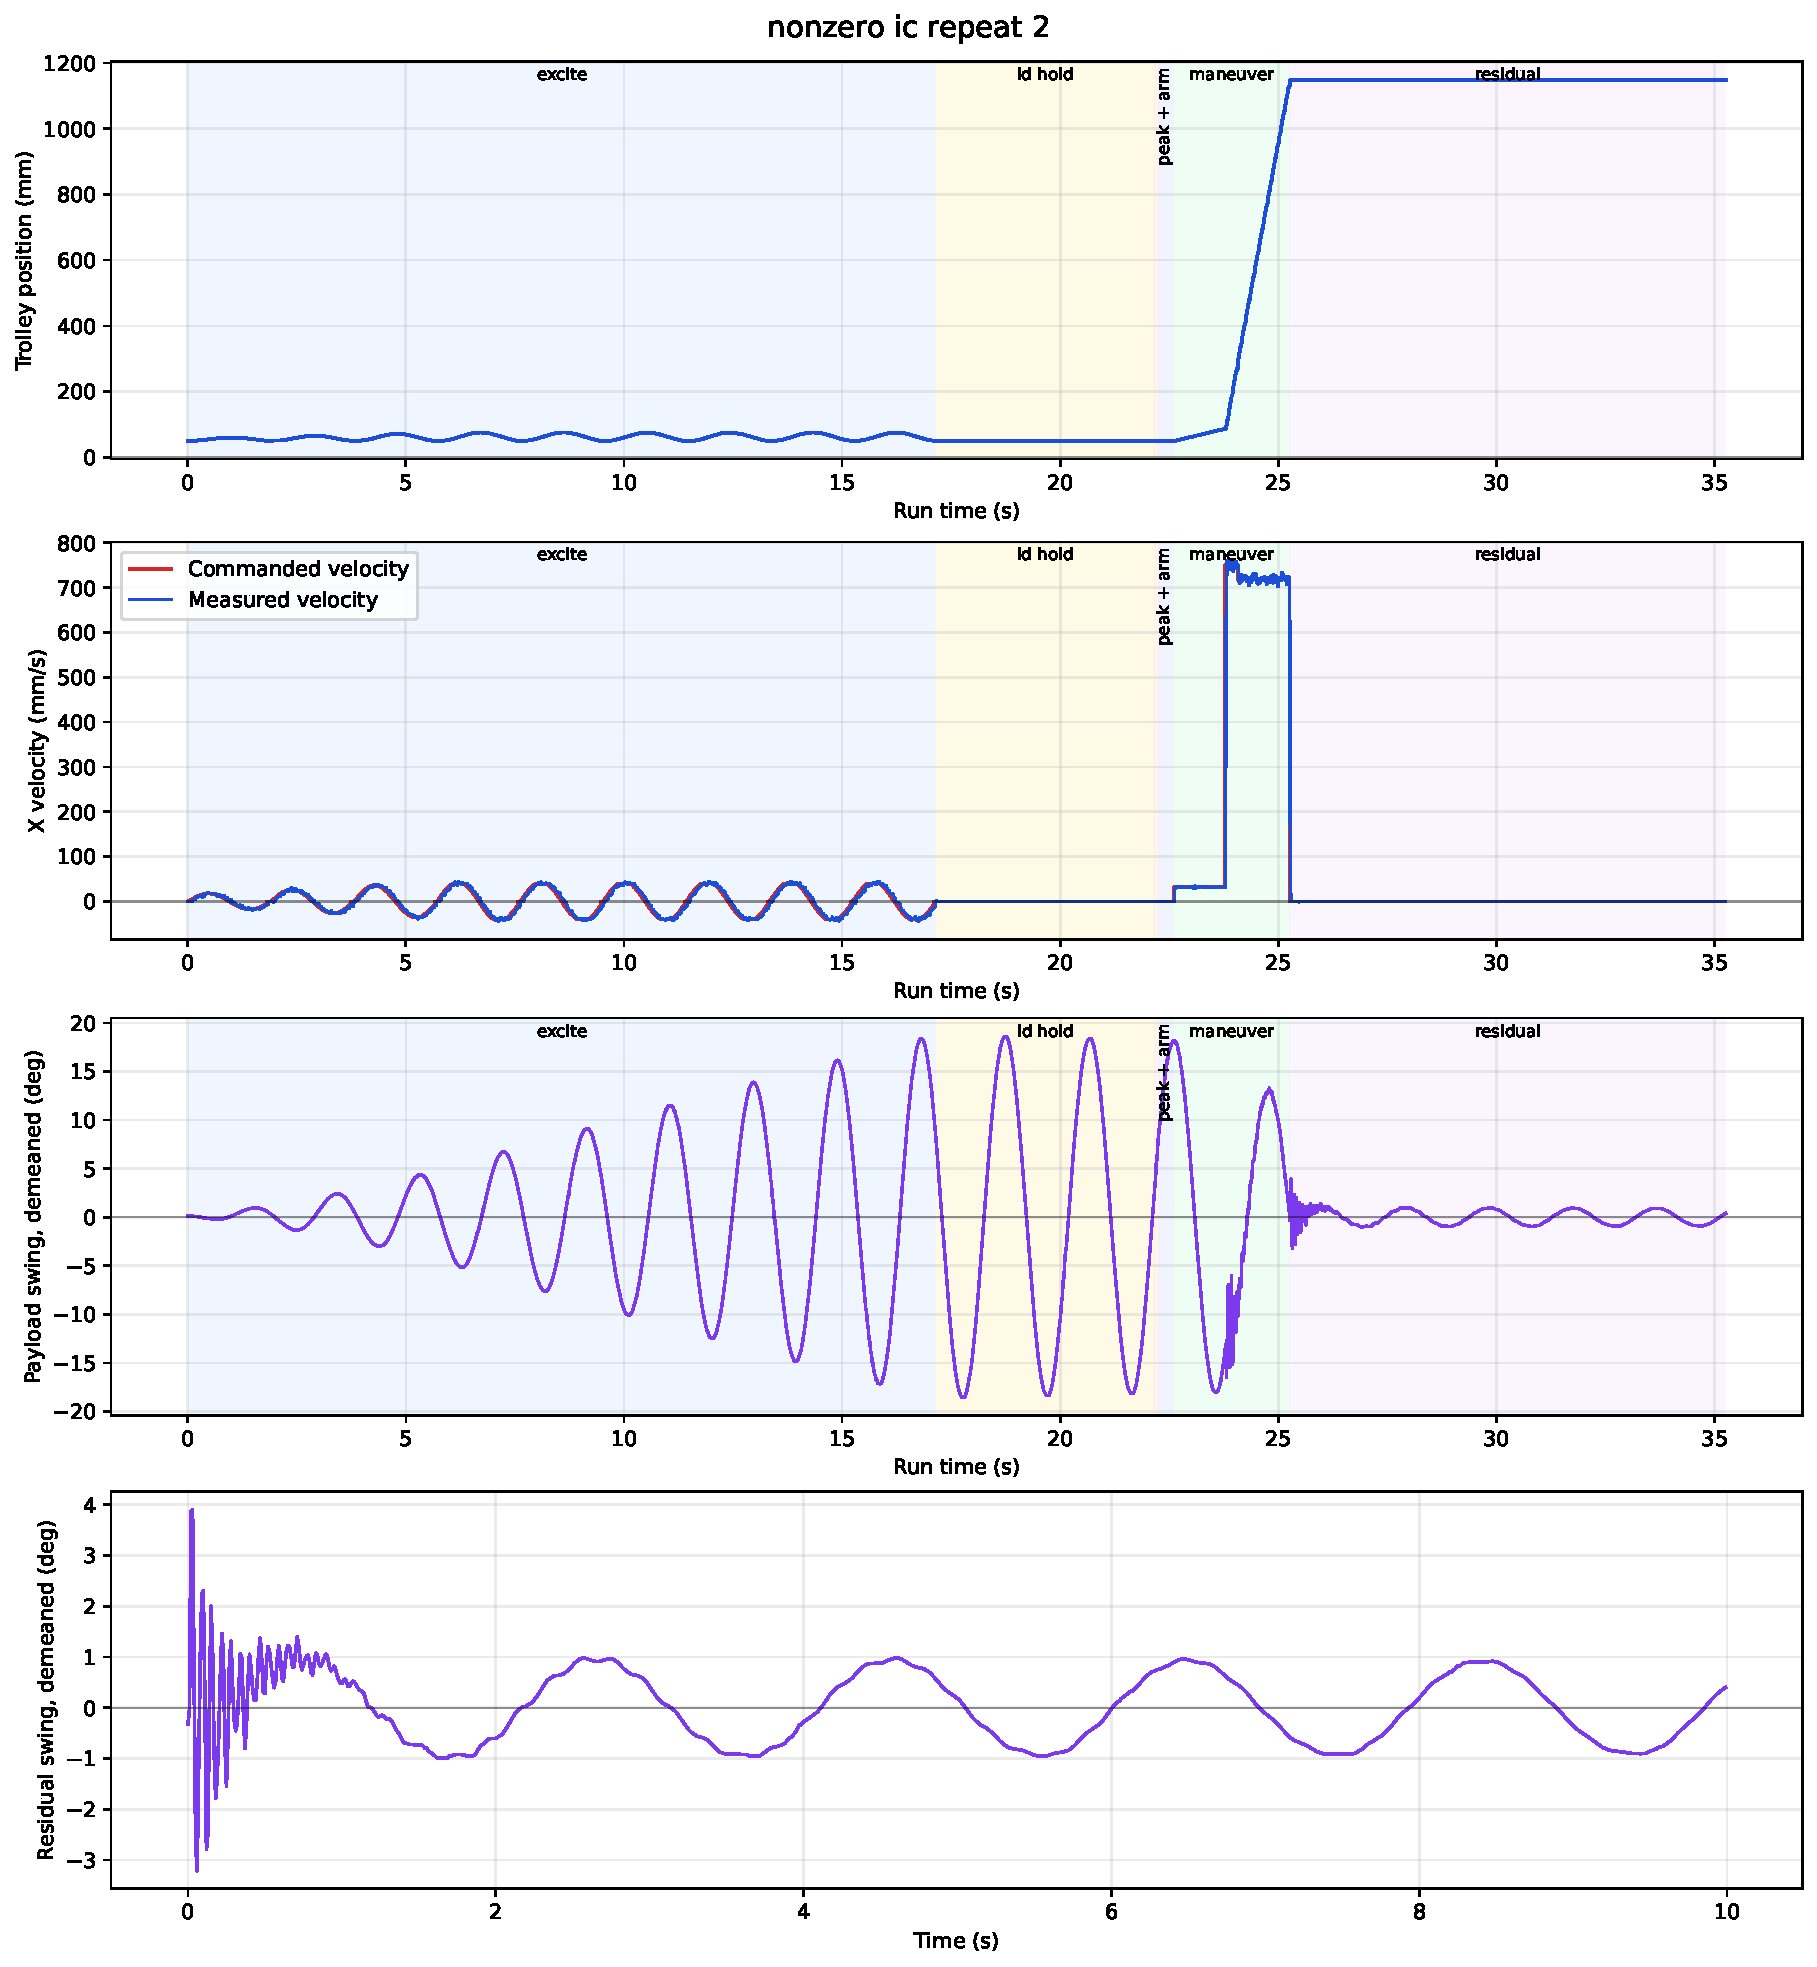
\includegraphics[width=0.98\textwidth]{nonzero_ic_repeat_2.pdf}
    \caption{Representative adaptive nonzero-initial-condition experiment
    (Rep.~2).  From top to bottom: trolley position, commanded and measured
    trolley velocity, demeaned payload swing over the complete experiment,
    and demeaned residual swing.  The method identified
    $\widehat{\omega}_{\mathrm f}=3.24960~\mathrm{rad/s}$ and applied the
    finite-amplitude-corrected value
    $\widehat{\omega}_0=3.27109~\mathrm{rad/s}$.  The $1100~\mathrm{mm}$
    maneuver reached $750~\mathrm{mm/s}$ and reduced the fitted fundamental
    swing amplitude from $18.579^{\circ}$ to $0.937^{\circ}$.}
    \label{fig:nzic_repeat_2}
\end{figure*}

